
%
%  $Description: Author guidelines and sample document in LaTeX 2.09$
%
%  $Author: Dillon Lareau $
%  $Date: 12/12/2016 $
%  $Revision: 1.0 $
%

\documentclass[times, 10pt,twocolumn]{article}
\usepackage{latex8}
\usepackage{times}
\usepackage{graphicx}
\graphicspath{ {images/} }

%\documentstyle[times,art10,twocolumn,latex8]{article}

%-------------------------------------------------------------------------
% take the % away on next line to produce the final camera-ready version
\pagestyle{empty}

%-------------------------------------------------------------------------
\begin{document}

\title{Citation and Affiliation Networks in Academia }

\author{Gabriel Hobeika\\
ECE, Carnegie Mellon University\\ Pittsburgh, PA, USA\\
gph@andrew.cmu.edu\\
% For a paper whose authors are all at the same institution,
% omit the following lines up until the closing ``}''.
% Additional authors and addresses can be added with ``\and'',
% just like the second author.
\and
Dillon Lareau\\
ECE, Carnegie Mellon University\\ Pittsburgh, PA, USA\\
jlareau@andrew.cmu.edu\\
}

\maketitle
\thispagestyle{empty}

\begin{abstract}
Citation networks in academia can provide insight into the success of papers, as well as the success of their authors. Furthermore, trends in paper citations can point to new rising ideas, enlighten our understanding of relationships between universities and other institutions and between disciplines. While there has been some research into academic citation networks, we feel the need to go deeper. We will browse databases of papers, scrape relevant information to create networks, and then analyze those networks to identify what creates a successful paper, as well as any interesting relationships between institutions, journals and cross discipline works. We will compare our work and the network data that we find against other metrics that measure success. We will then see if any network-science based metrics help us predict or identify success in the traditional networks.
\end{abstract}


%-------------------------------------------------------------------------
\Section{Introduction}
Our project will be looking at network trends in the world of academia. More specifically, we seek to analyze citations and references between different authors, disciplines, and fields of study. We hope to be able to identify what marks ‘success’ in different ways throughout academia as described by our questions below.

%-------------------------------------------------------------------------
\Section{Motivation}
Firstly, we specifically want to analyze what types of colleges and universities are most likely to have authors cross collaborate. We also hope to identify whether things like ranking, endowment, or school type (private vs. public) determine anything about whether academics are likely to work together in the future. We also want to see how ranking of university is related to institutions that they work with, and see if we can devise a way to rank those institutions based on their network position.\\

Secondly, we want to see what journals are most likely to cite one another. We are specifically interested in whether the prestige of a specific journal affects the ratio of self-citing versus inter-journal citing. We also want to see what, if any implications, our network can show for conferences, and one-off publications.\\

Thirdly, we want to identify how network statistics relate to author success. More specifically, we would like to evaluate how citations networks, and collaboration networks affect metrics like H-index. This will give us an idea of what authors should do in order to increase their H-index in the future and should help us identify when an author is poised to be more successful and get a higher H-index. \\

Lastly, we want to be able to look at some of our previous subjects across time. For instance, we would like to see how an author’s position in the network at the time of publishing a paper relates to their success in future publications contained in the network that we created. \\

Networks are fundamental to each of these goals. For each of the goals, in order to identify the relationships between papers on a large scale we will have to create networks that identify what papers cited, where those papers are from, whom they reference, and what connections do the papers and authors have to the outside world.


%-------------------------------------------------------------------------
\Section{Prior Work}
We have viewed some authors previous work in the field of academic paper citation networks. \\

One of our primary inspirations titled “A Century of Physics” [1], looks at 100 years of papers in the physics world through web of science and analyzes the long-term impact of different publications based on their reference data. It shows how publications and papers can have an impact over a range of time.\\

Our work differs from that paper, as we are generally looking at small-scale in terms of time when compared to the 100 years of physics papers. We want to be able to identify what will cause an impact, not what has caused an impact in the past. Additionally, as the title implies, “A Century of Physics” focuses just on the physics discipline. It is our hope to find data that can apply to multiple disciplines, and cross discipline work. We have found  acquiring paper data for many disciplines is a complex process. In this paper we have been able to look at collaborations between institutions accross all disciplines, but not at many disciplines at the paper-level. \\

We also looked at Newman’s [2] approach in “Finding community structure in networks using the eigenvectors of matrices.” This paper was helpful in helping us analyze the citation information from a community perspective. Additionally, Newman has a publicly available dataset for his work, which we do not directly use in our work, but that we have viewed to see how networks are sometimes structures when applied to academic citations and collaborations.\\

We differ from Newman, as we are not just concerned with communities in academia, but a concept of success. As such, we are interested in more detailed information about the papers themselves, and what topics they cover, not just the citations and cross-references between different academics. \\

We want to focus on broad analysis of the networks in academia, over the whole spectrum of academia. Most other work in the field focuses on one metric, or one quantitative finding. Our work seeks to define the abstract relationships across academia, between journals, institutions, and even between authors themselves. We hope that our broad scope will give us insights into success not previously explored.

%-------------------------------------------------------------------------
\Section{Approach}
Our approach relies on our attempts to acquire a wide range of data. As highlighted before, we need many data to evaluate the metrics we want, and as such, we are going to need to figure out ways to extract data from existing databases for usages that they have not catered to before.\\

Our approach has evolved throughout the completion of this project. For the first part of the project we had to develop ways to scrape data, and collect data from databases who's intended purpose was not to be data-mined in the way we have intended. We found a way to do bulk data collection from the SAO/NASA database. This allowed us to gather papers and the citations between them. We manually had to query the Scopus database to find collaborations between institutions. This is because the Scopus API was not developed with large-scale network creation in mind. \\

From the SAO\NASA Database we started with a subset of 10 papers. From those papers, we got all of the papers that were cited. We then went one level detail, and again got all of the papers those paper's cited. This allowed us to  use a large set  of more than 15000 papers. These papers had more than 35000 unique authors. As such, we had to limit the dataset when creating a network from it. \\

From Scopus, we began by looking at Carnegie Mellon University. We identified the top 50 collaborating institutions of CMU. A collaborating institution is defined as one where an author from that institution had directly coauthored a paper with another author from a different institution. We then looked at the top 150 Collaborating institutions of the institutions in that list. This left us with over 700 institutions, with tens of thousands of collaborations between them.  We faced a limitation here, as Scopus was not designed to be queried in the two-deep fashion we had been using. It is useful for looking up one paper, or one institution, but is not developed to find a network around them.\\

We then setup networks from the raw data we collected. Using the SAO/NASA database results, we connected the authors of the papers. In one network, we started with Authors of papers, we then connected those authors to the authors of the cited papers. The In-edges of that network measured a citation by another author. The out edges measured a citation of another author. We also created a collaboration network. For the collaboration network, we had authors as nodes ones again. This time, edges were omnidirectional. A collaboration edge was added for each co-authorship between an author and another author. We also created a network of journals from the SAO/NASA database. For that network, we used the journal a piece was published in as the nodes. We then added edges for citations to other journals that were used. For the institution networks, we started with the Institution as the nodes. We then added weighted edges, with the numbers of collaborations between the institutions.  \\

We then performed simple analysis on these networks. We looked at the degrees of the edges in the author networks to try to garner some simple intuition about the authors. For instance, the highest in-degree's in the network should indicate the most cited author, and the most worked-with author. We used these as initial measures of success. We performed the same analysis on the institutions network. We then did community analysis using Gephi to detect communities on all the networks. The results of the analysis is discussed in the experimental results section. \\

After we had performed the rudimentary success analysis, we looked to get real-world metrics of success. For authors, we looked at their H-Index. We chose H-Index to look at, as it is currently one of the most widely used measures of success that looks both at an authors contributions and their impacts. Similarly from journals, we looked at the H-5 indexes of the journals as provided by google scholar. Lastly, for the institutions, we looked at both the ARWU world rankings, and the Times world rankings to identify the success of the institutions in teh real world. We compared these metrics to the network-statistics of the networks we had created. We tried to identify correlating trends to ascertain if networks could tell us anything about academia. \\

Lastly, we attempted to generate our own success metrics. We tried to look at the ranking of the nearby-nodes within our networks to ascertain any knowledge about the potential ranking of the focus node. Our results and full process for this analysis are discussed within. 
%-------------------------------------------------------------------------
\Section{Results}

\SubSection{Experimental Setup and Practical Results M1}
Through our initial research and data gathering, we have found that most papers include a large number of citations, between 10 and 20 citations a paper. We gathered our initial set of papers from the SAO/NASA Astrophysics Data System [3]. We started by looking at 100  starting papers. This generated a network that was far too large to visualize, as it balooned to many thousands of papers after looking at the citations. Because the number of citations was so large, we had to scale down our network in order to run some simulations on it on Gephi. What we found in our citation network was rather interesting. The network properties are in table 1.

\begin{table}[]
\centering
\caption{My caption}
\label{my-label}
\begin{tabular}{|l|l|}
\hline
Papers                 & 6808  \\ \hline
Citations              & 10607 \\ \hline
Average Degree         & 3.116 \\ \hline
Number Communities     & 19-21 \\ \hline
Clustering Coefficient & 0.047 \\ \hline
\end{tabular}
\end{table}

This dataset ended up not being used in our final results, but gave us an initial way to mine for data that we built off of for the remainder of the project.

\begin{figure}[h]
   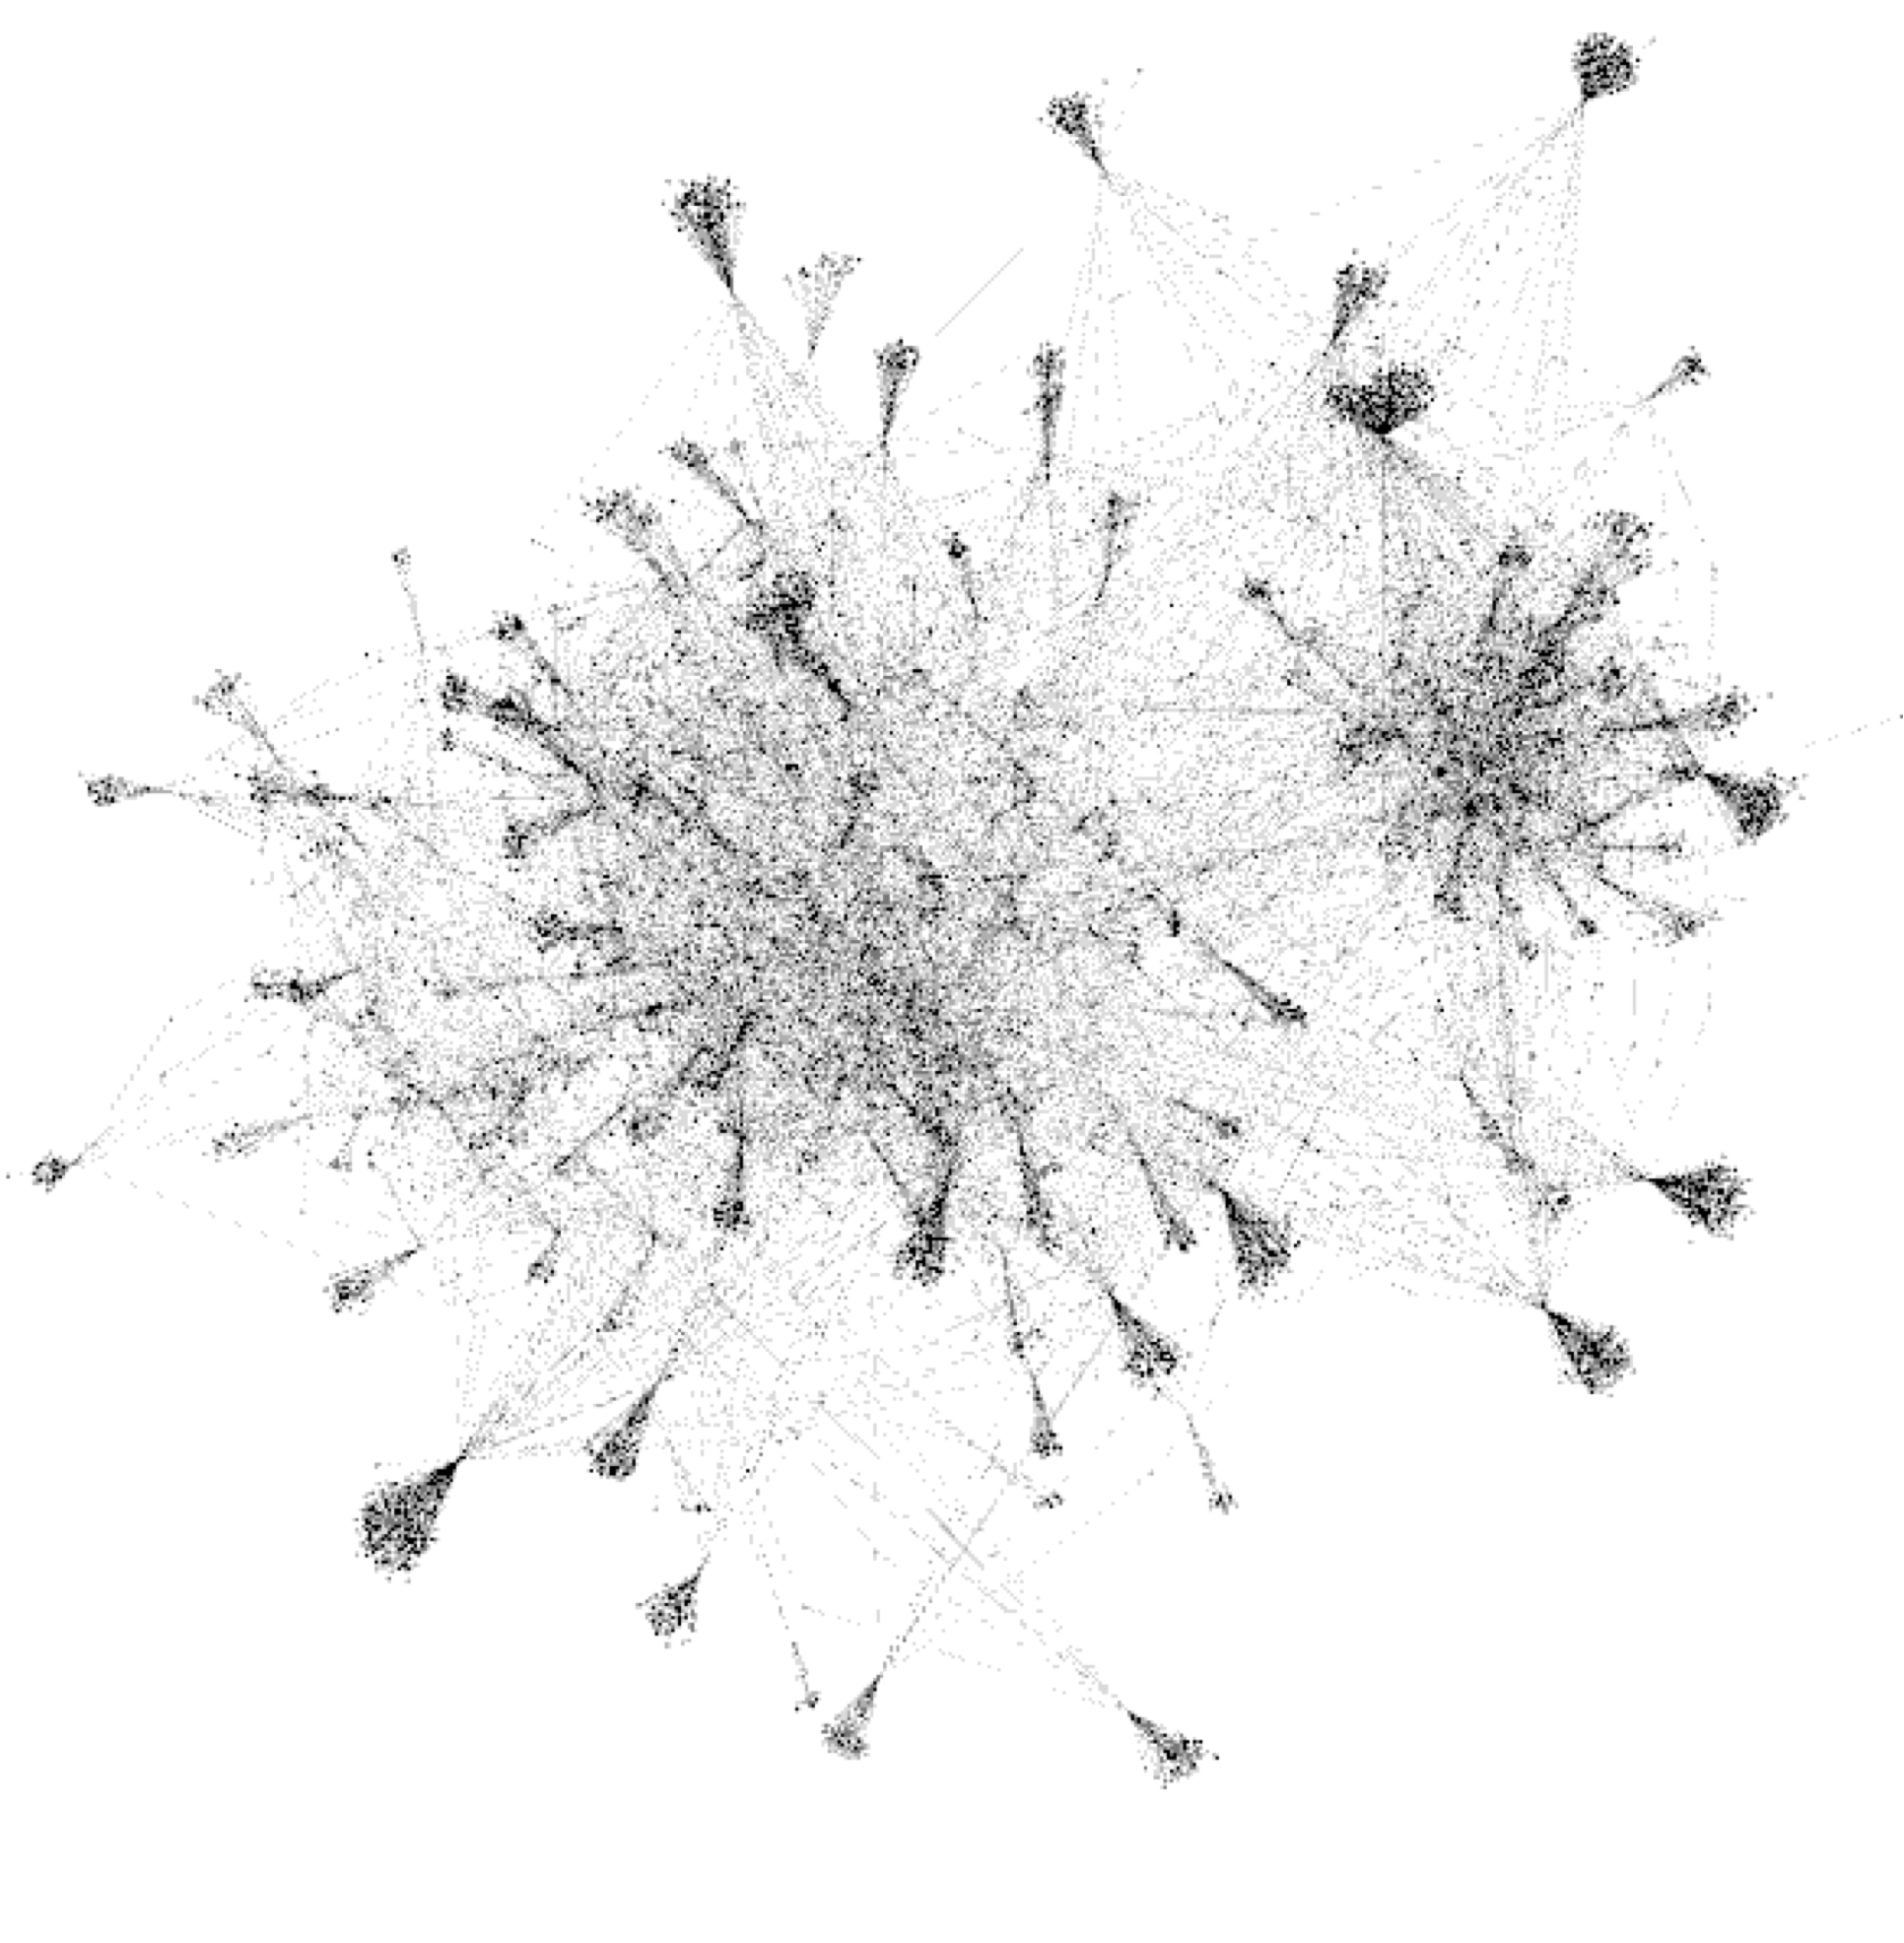
\includegraphics[width=8cm]{figure1.png}
   \caption{Example of caption.}
\end{figure}

%-------------------------------------------------------------------------
\SubSection{Experimental Setup and Practical Results M2 + M3}
After getting that initial research from M1, we decided to narrow down what we were looking for, and we split up our data collection so that we could accomplish all of our goals. What we looked to create were: \\
1. A collaboration network between authors who have at least 10 publications \\
2. A citation network between journals based on the data collected regarding author citations.\\
3. A collaboration network between institutions that have at least 50 papers each.\\

We managed to obtain more data out of the SAO/NASA Data system. Using the data that we obtained, we created both a collaboration network between authors who have at least 10 publications, and a citation network between journals based on the data that lead to the author network. To create these networks we followed the model outlined in the approach.  \\

Firstly, we looked at the author collaboration network [Figure 2].  Our first approach was to look at the communities within this network. We found a high value of modularit and a high number of communities, with the normal random community finding algorithm used in Gephi. The baseline network statistics are included in [table 2] \\

\begin{figure}[h]
   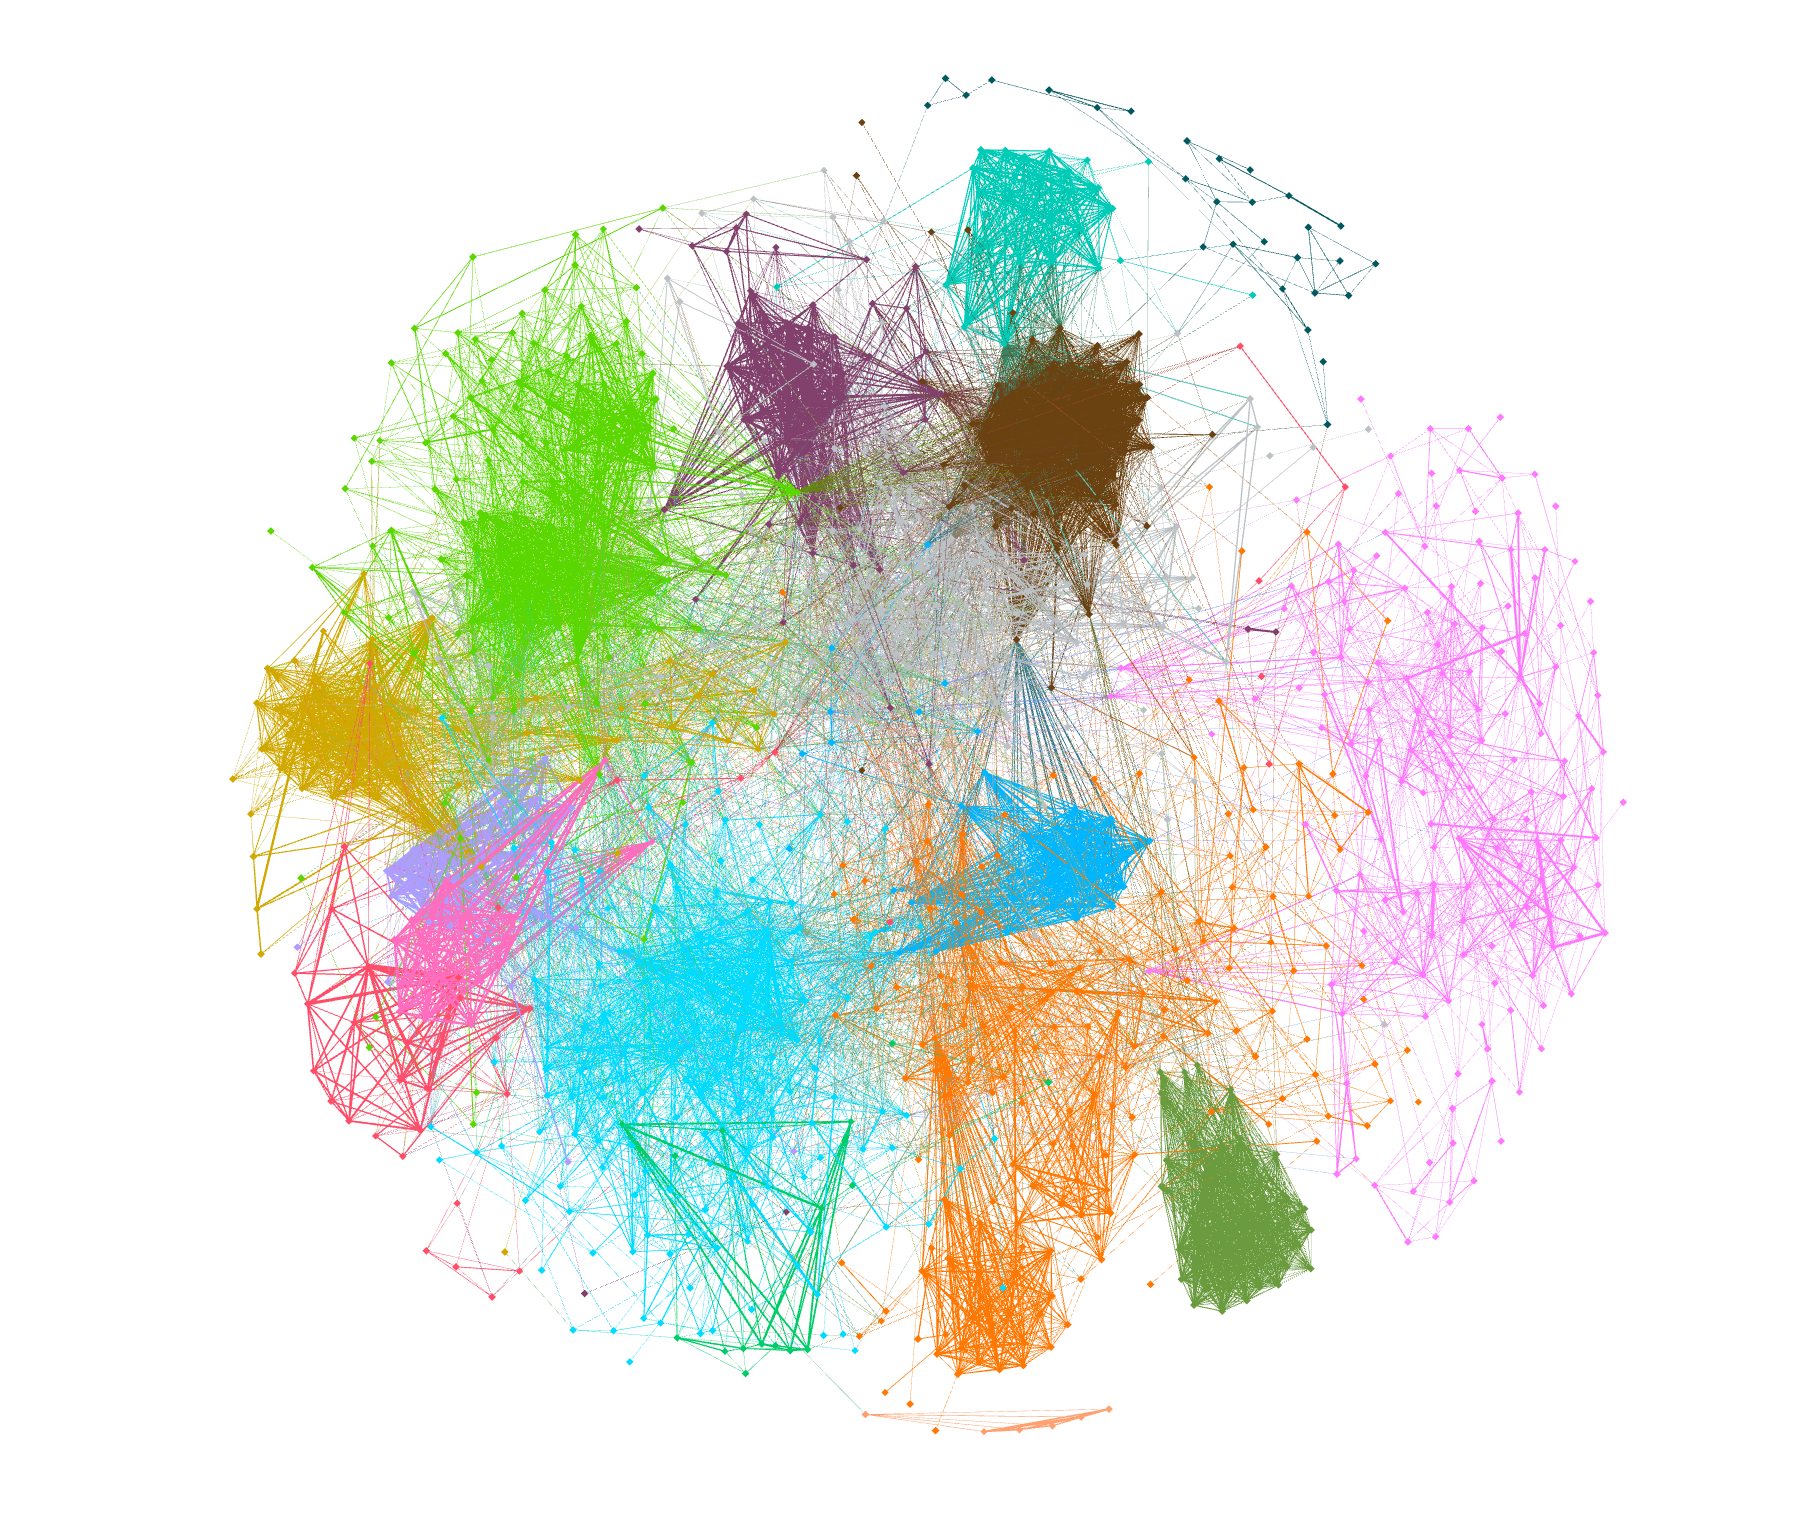
\includegraphics[width=8cm]{figure2.png}
   \caption{Example of caption.}
\end{figure}

\begin{table}[]
\centering
\caption{My caption}
\label{my-label}
\begin{tabular}{|l|l|}
\hline
Authors / Nodes      & 741   \\ \hline
Collaborations/Edges & 17185 \\ \hline
Average Degree       & 6.344 \\ \hline
Communities          & 13    \\ \hline
Modularity           & 0.721 \\ \hline
\end{tabular}
\end{table}

We identified that the communities within this network seemed to be based around authors that had all collaborated on one large paper. As such, the community structure was important which explains our high modularity value. The initial intuition this gave us was to look for authors that had worked on those high-value large papers. \\

We found Gephi’s community analysis helpful in finding these specific authors. We have looked at this as one metric of success within our network; that is to say if an author collaborates on more than one ‘big’ papers, he must be a respected author. \\

Next, we looked at a journal citation network [Figure 3]. The figure is colored by community of the journal. The general properties of this network can be found in table 3. It was generated from the set of papers that made the author collaboration network. Unlike the author network, this network did not have a high modulatrity value. This means the communities discovered in this network are less important. In addition, it had a low level of communities, regardless of the resolution parameter. \\

\begin{figure}[h]
   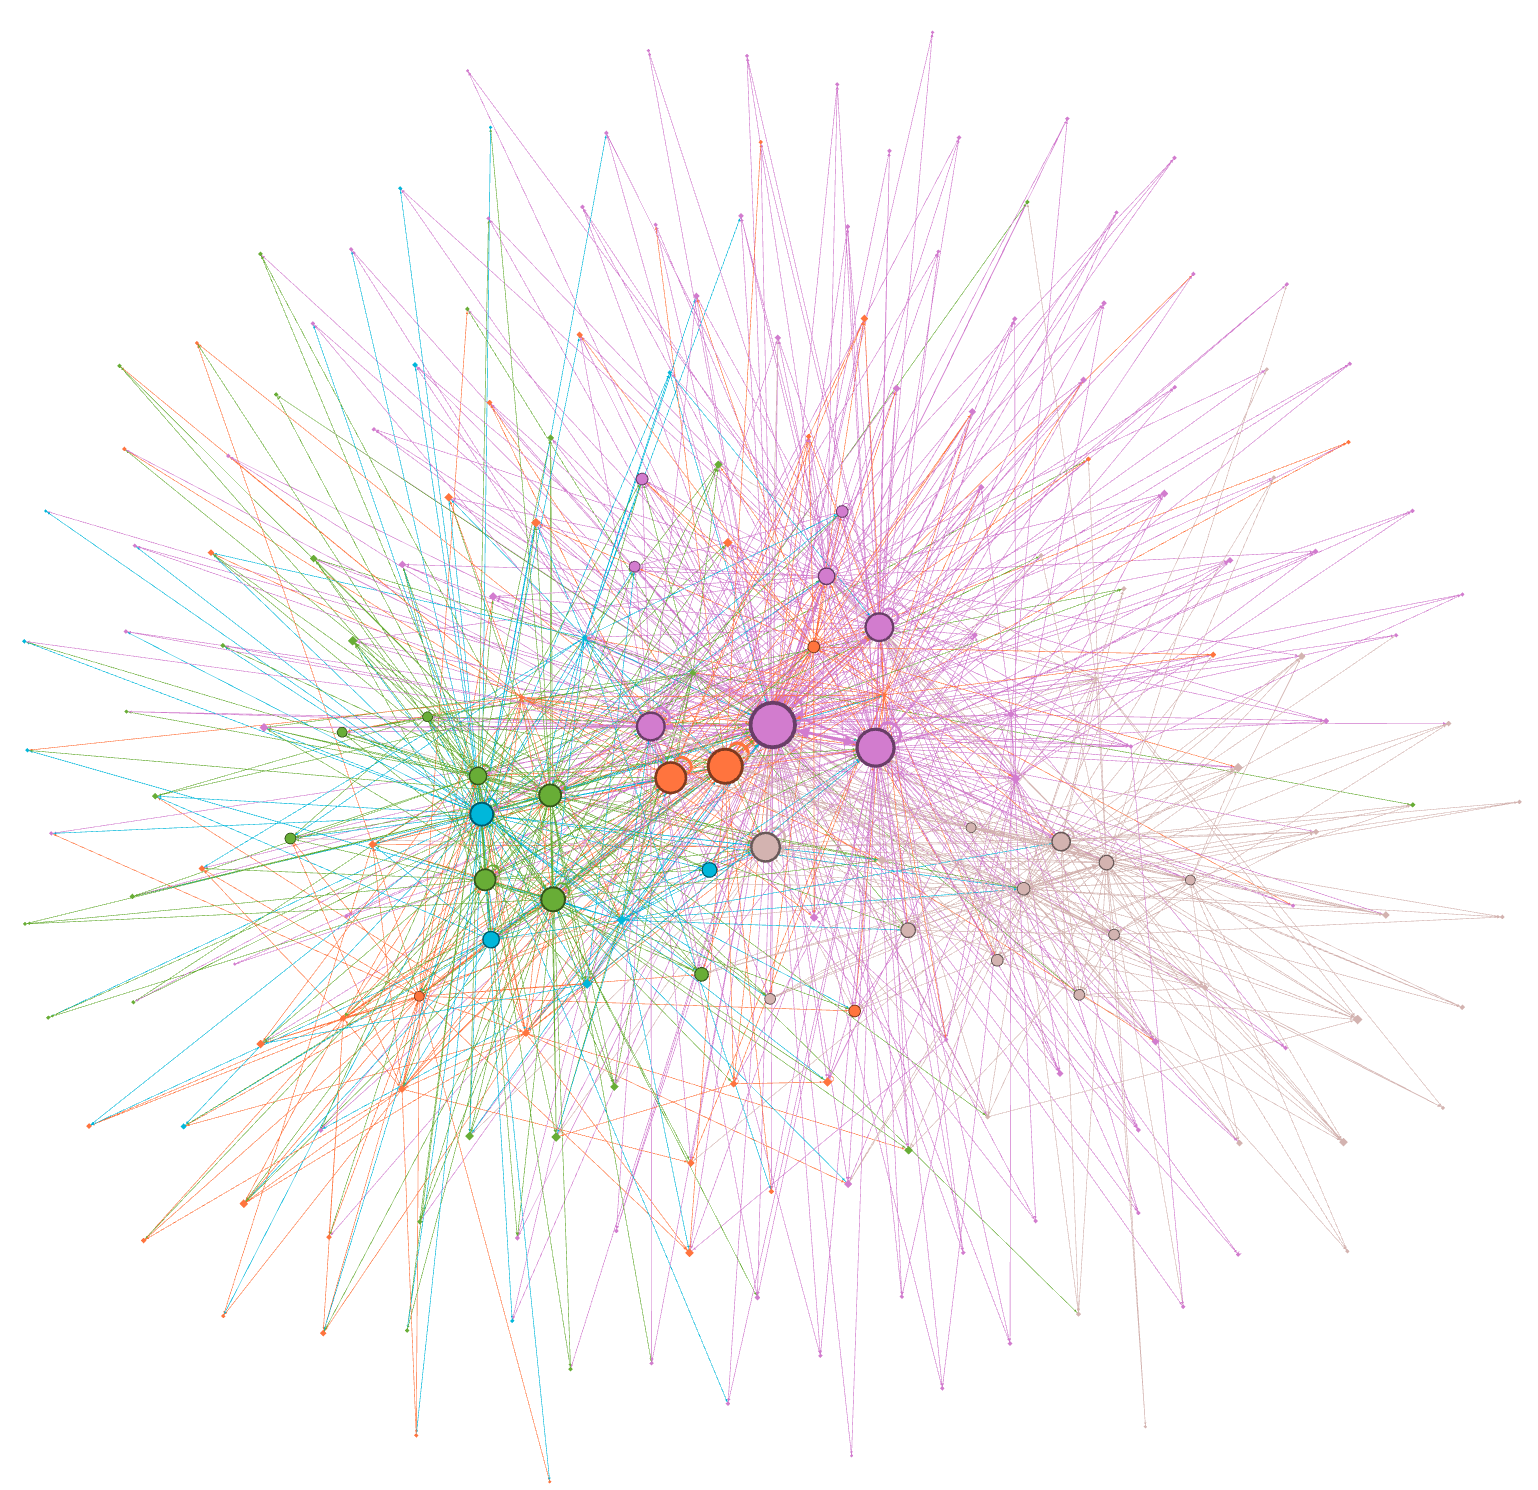
\includegraphics[width=8cm]{figure3.png}
   \caption{Example of caption.}
\end{figure}

\begin{table}[]
\centering
\caption{My caption}
\label{my-label}
\begin{tabular}{|l|l|}
\hline
Journals               & 291   \\ \hline
Citation               & 13445 \\ \hline
Average Degree         & 6.344 \\ \hline
Number Communities     & 5     \\ \hline
Clustering Coefficient & .321  \\ \hline
\end{tabular}
\end{table}
\\

The interesting result we found was when we compared the network we generated to the H5-Index found on google scholar.[7] We found our most heavily cited journals, like the Astrophysics Journal, and the Monthly Notices of the Royal Astronomical Society also scored high on the H-index rating. We think our measure of success can be slightly different from H5-Index, where H-Index looks at citations over time; our rating looks at bursts of citations in one particular field. For this particular field, astrophysics, our metrics did not completely align with H-Index. In particular, The Astrophysical Journal scored higher on our metrics than Science or Nature, which both have much higher H-Indexes. We believe looking at burst citations may be valuable in establishing better success metrics for our papers.\\

In milestone 3, we refined these networks somewhat. We looked at physics collaborations vs astronomy collaborations during milestone 3. What we found was somewhat interesting. We started with the same amount of papers, and roughly the same amount of author [table 4] \\

    \begin{tabular}{ | l | l | l |}
    \hline
    Discipline: & Astronomy & Physics \\ \hline
    Papers & 16,416 & 17,818  \\ \hline
    Authors & 37,063 & 35,724 \\ \hline
    $> 10$ & 1,150 & 339 \\ \hline
    $> 20$ & 318 & N/A \\ \hline
    \end{tabular}\\

Using this data, we observed some interesting differences between the astronomy and physics datasets. The first and most obvious difference is the number of authors with $>$10 publications. Significantly more authors in astronomy seemed to have worked on that many publications within this collaboration network. \\

This was interesting, as we had previously figured that the structure of the citation networks would not vary that greatly between disciplines. This set of data, however, shows something different. It suggests that with physics papers there are less prolific authors among the data that we were able to sample, than astronomy datasets. \\

The physics dataset, filtered on 10 papers, also is not a completely connected network. The image below shows the comparative sparsity of the dataset when compared to the above images of the astronomy data. The image shows that in physics, like astronomy, there are clearly defined communities. That is to say that we identified that some authors are still more likely to work together and to cite each other and that within physics there are still some prolific authors. \\

We have also looked at H-Index as a success metric [6], both globally and measured in our own citation network. We compared this universal success metric to network factors, like node degree, K-Core, and centralities. We have included graphs with this paper to show the relevant trends that we have found. In summary, those trends are generally inconclusive. We were however able to find some interesting results when looking at collaboration within our network when compared to the H-Index of the network. \\

\begin{figure}[h]
   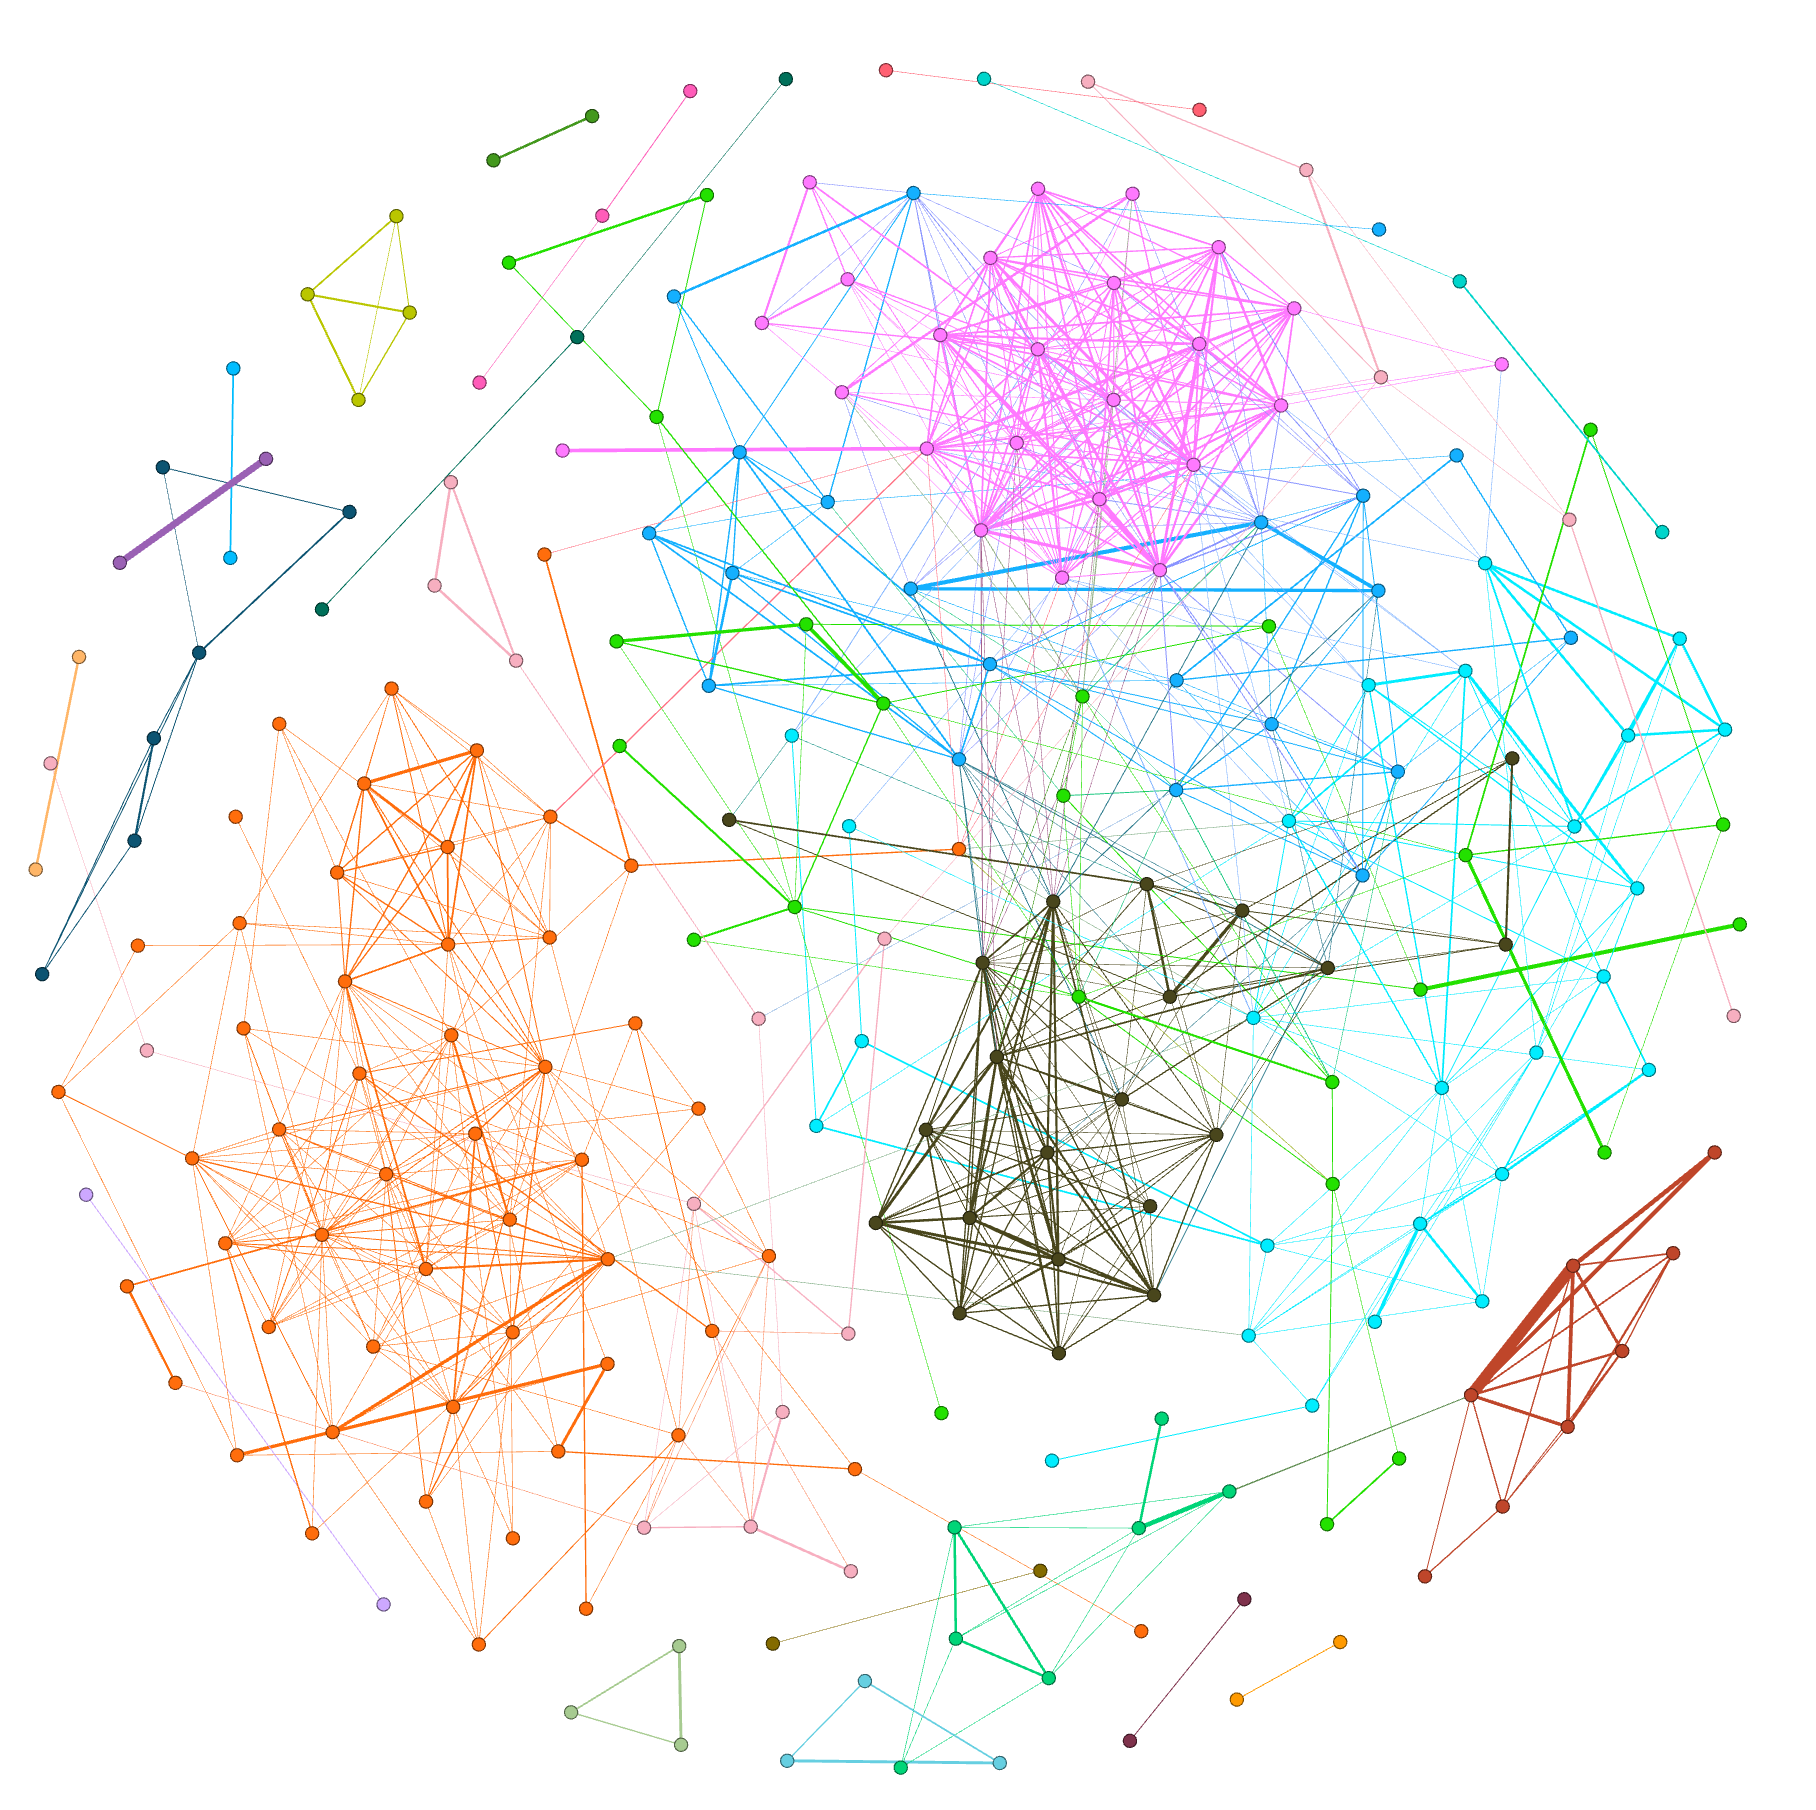
\includegraphics[width=8cm]{figure4.png}
   \caption{Example of caption.}
\end{figure}

As mentioned before, our most significant result when looking at H-index relative to the paper networks, was H-index to degree of collaborations. The graph [Figure 5] has a high degree of certainty ($R^2 = 0.8491$)  \\

\begin{figure}[h]
   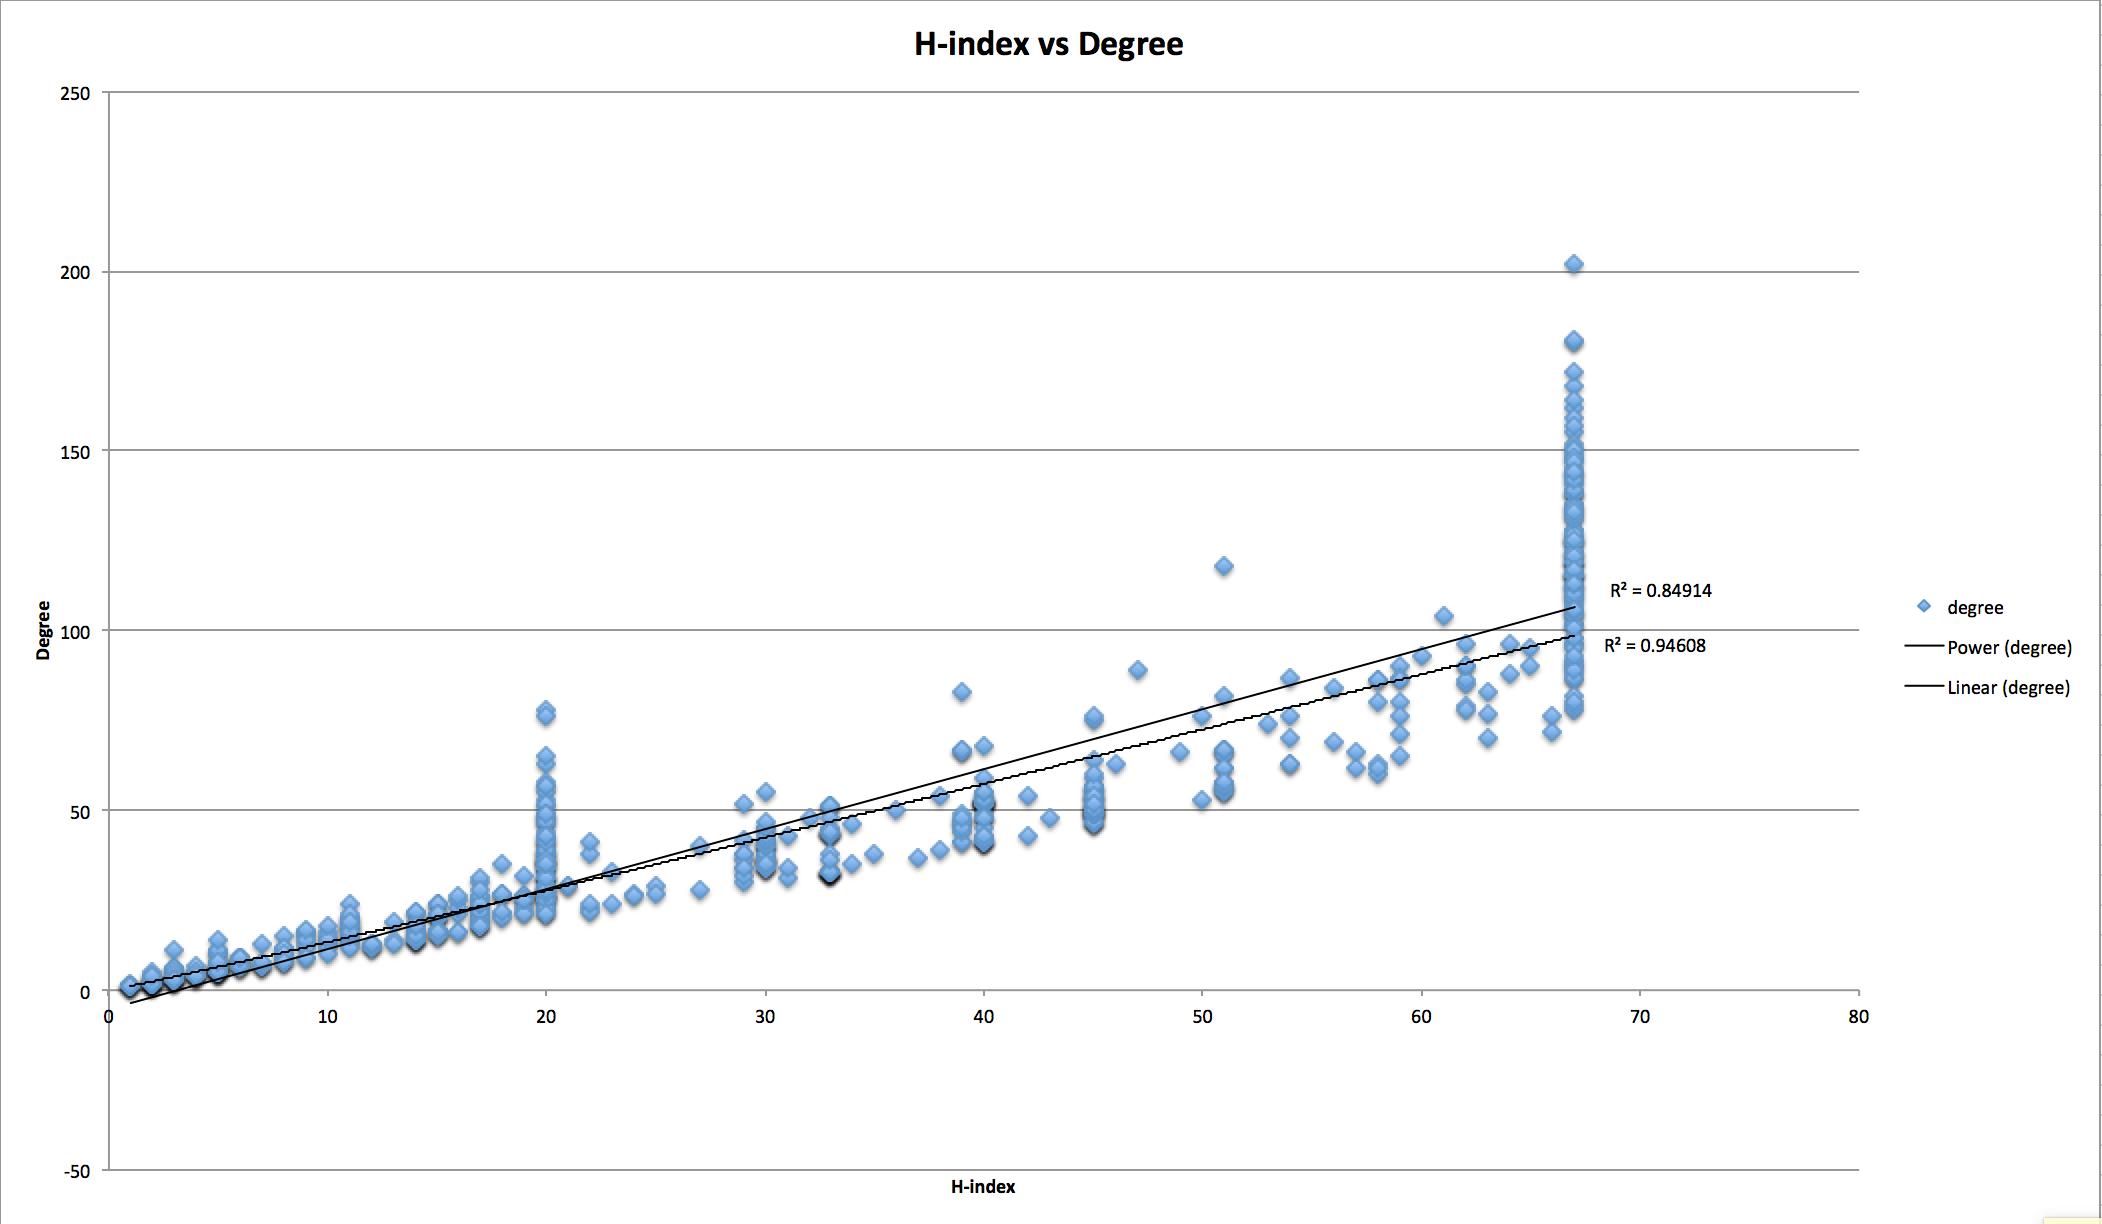
\includegraphics[width=8cm]{figure5.png}
   \caption{Example of caption.}
\end{figure}

This graph shows H-index on the x-axis with degree on the y-axis. This is the most highly correlated graph we have found. What we can identify from this is that when an author collaborates heavily, and works with a diverse array of authors, they will be more likely to score high on the universal metric of h-index. \\

We believe this has some rational backings: first of all, if an author collaborates more, they may have published more papers. Publishing papers has a factor in h-index as it measures productivity of paper writers. Also, if a professor’s work is collaborated on by other professors, those professors may self-cite their work in other papers. This will lead to the second requirement of H-index, citations, to be accomplished more easily. \\

The last network we generated drew from a different source. We used SCOPUS [4], which is one of the largest citation databases, in order to find the top 150 collaborating institutions, from 50 starting institutions. We came to this method of data collection, because we found that institutions typically have collaborations and citations with a very large number of other institutions. To try to grab all of the collaborations would be near impossible. We figured the top 150, which typically meant more than 500 collaborations had occurred, would narrow down our data set to a manageable point, without removing too much specificity. \\

Still, when making this network [Figure 6], we found that we had almost 700 very inter connected institution nodes. As with the Journal Citation network, this collaboration network had a low level of modularity, and not a large number of communities. In fact, establishing a real community structure was almost impossible. We made sure to add weight to all of the edges, and when visualizing, made the most heavily connected nodes larger. \\

\begin{figure}[h]
   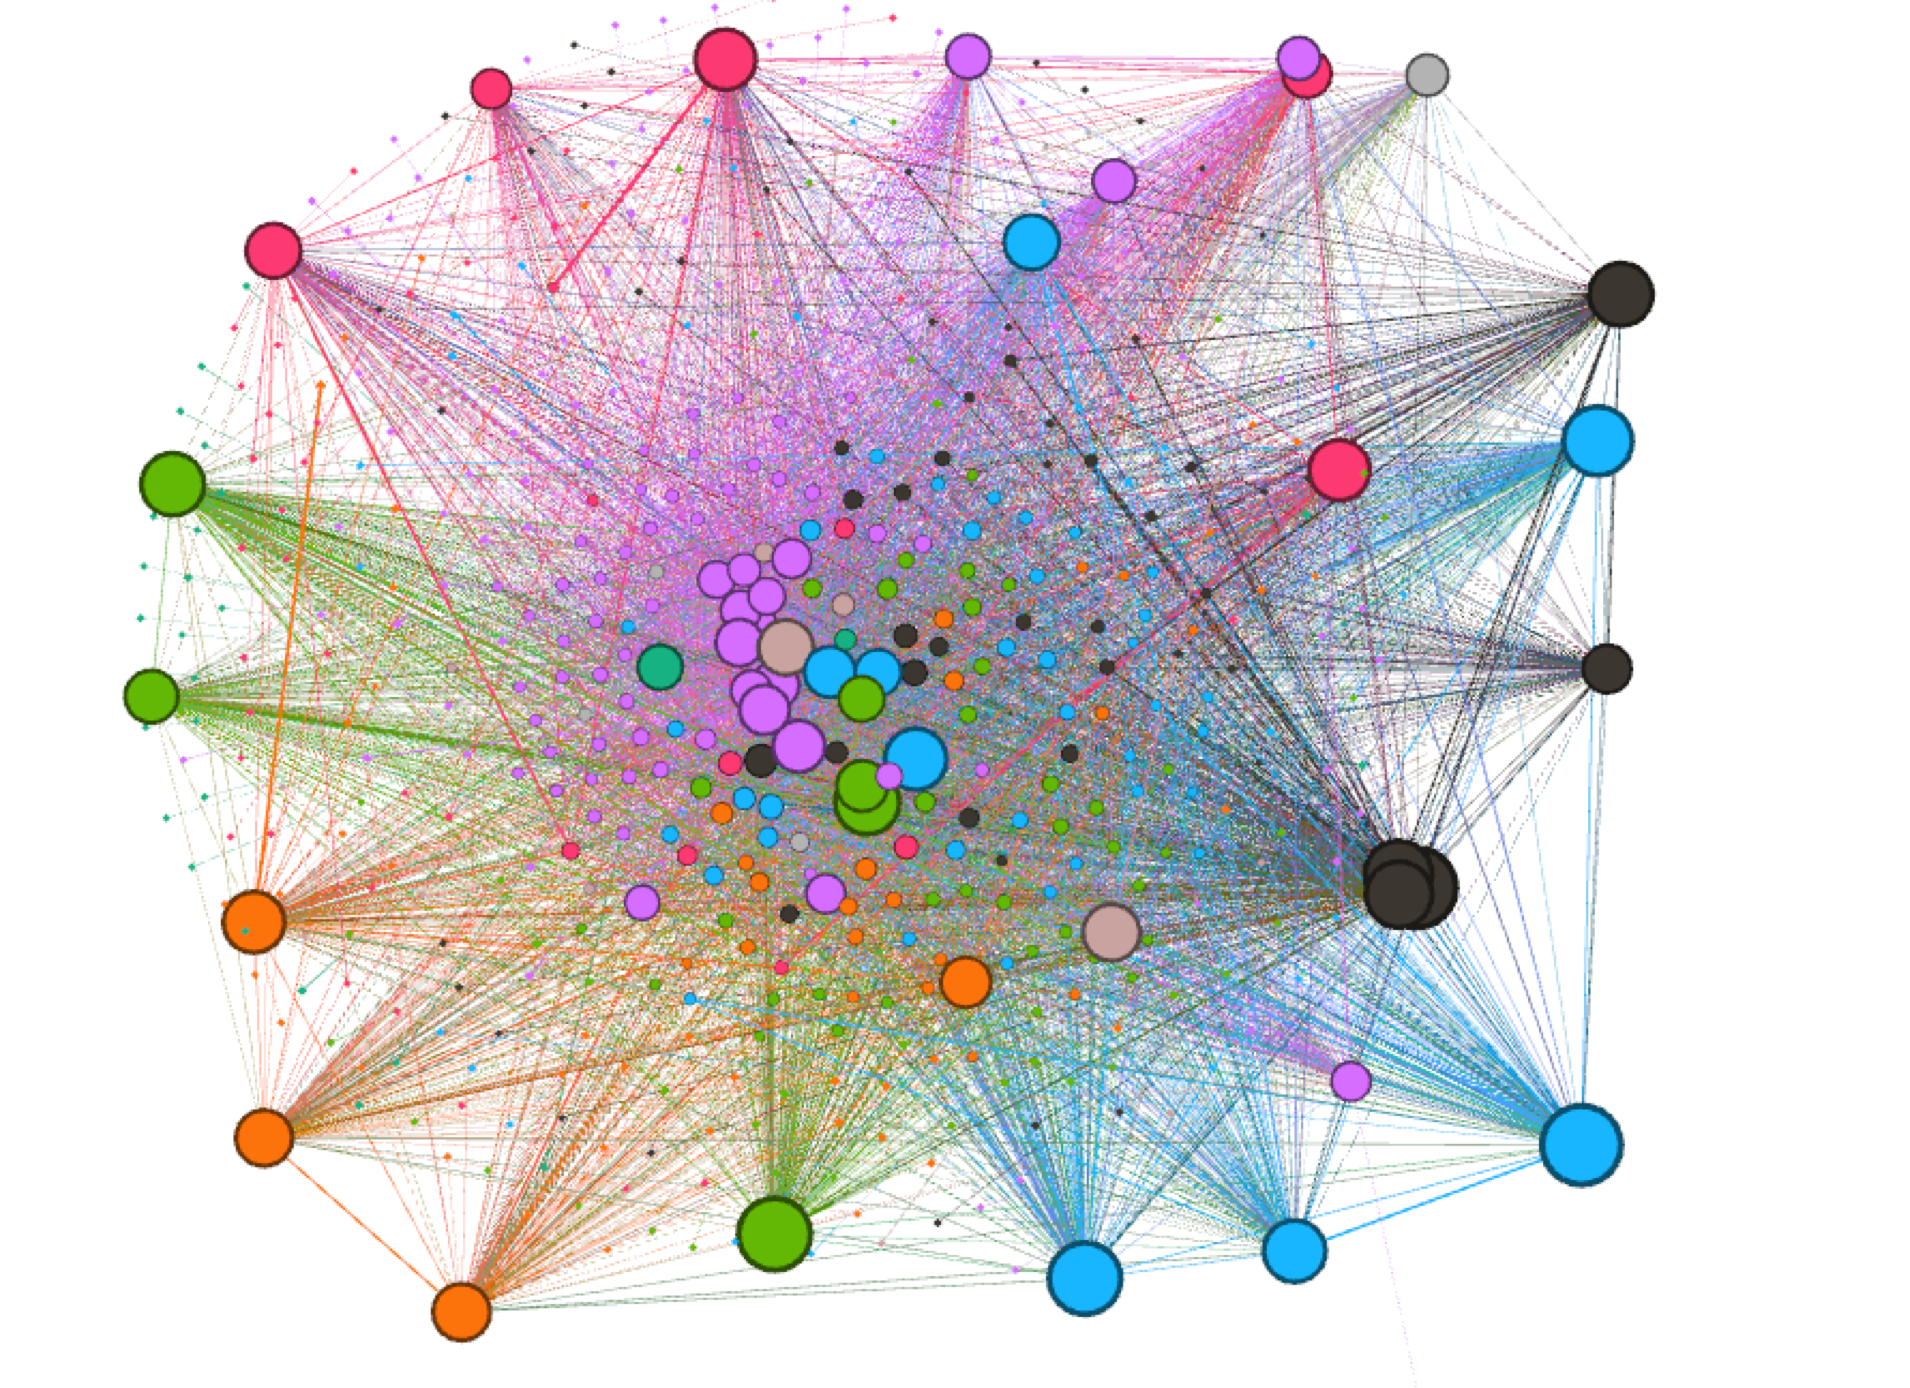
\includegraphics[width=8cm]{figure6.png}
   \caption{Example of caption.}
\end{figure}

Because of the method of data collection used, we also decided to filter out those nodes outside of the top 100 most connected nodes [Figure 7], most connected nodes for better visualization.  We found this showed the communities in a slightly nicer way, but the communities were still not heavily modular and did not inform us of much.    \\

\begin{figure}[h]
   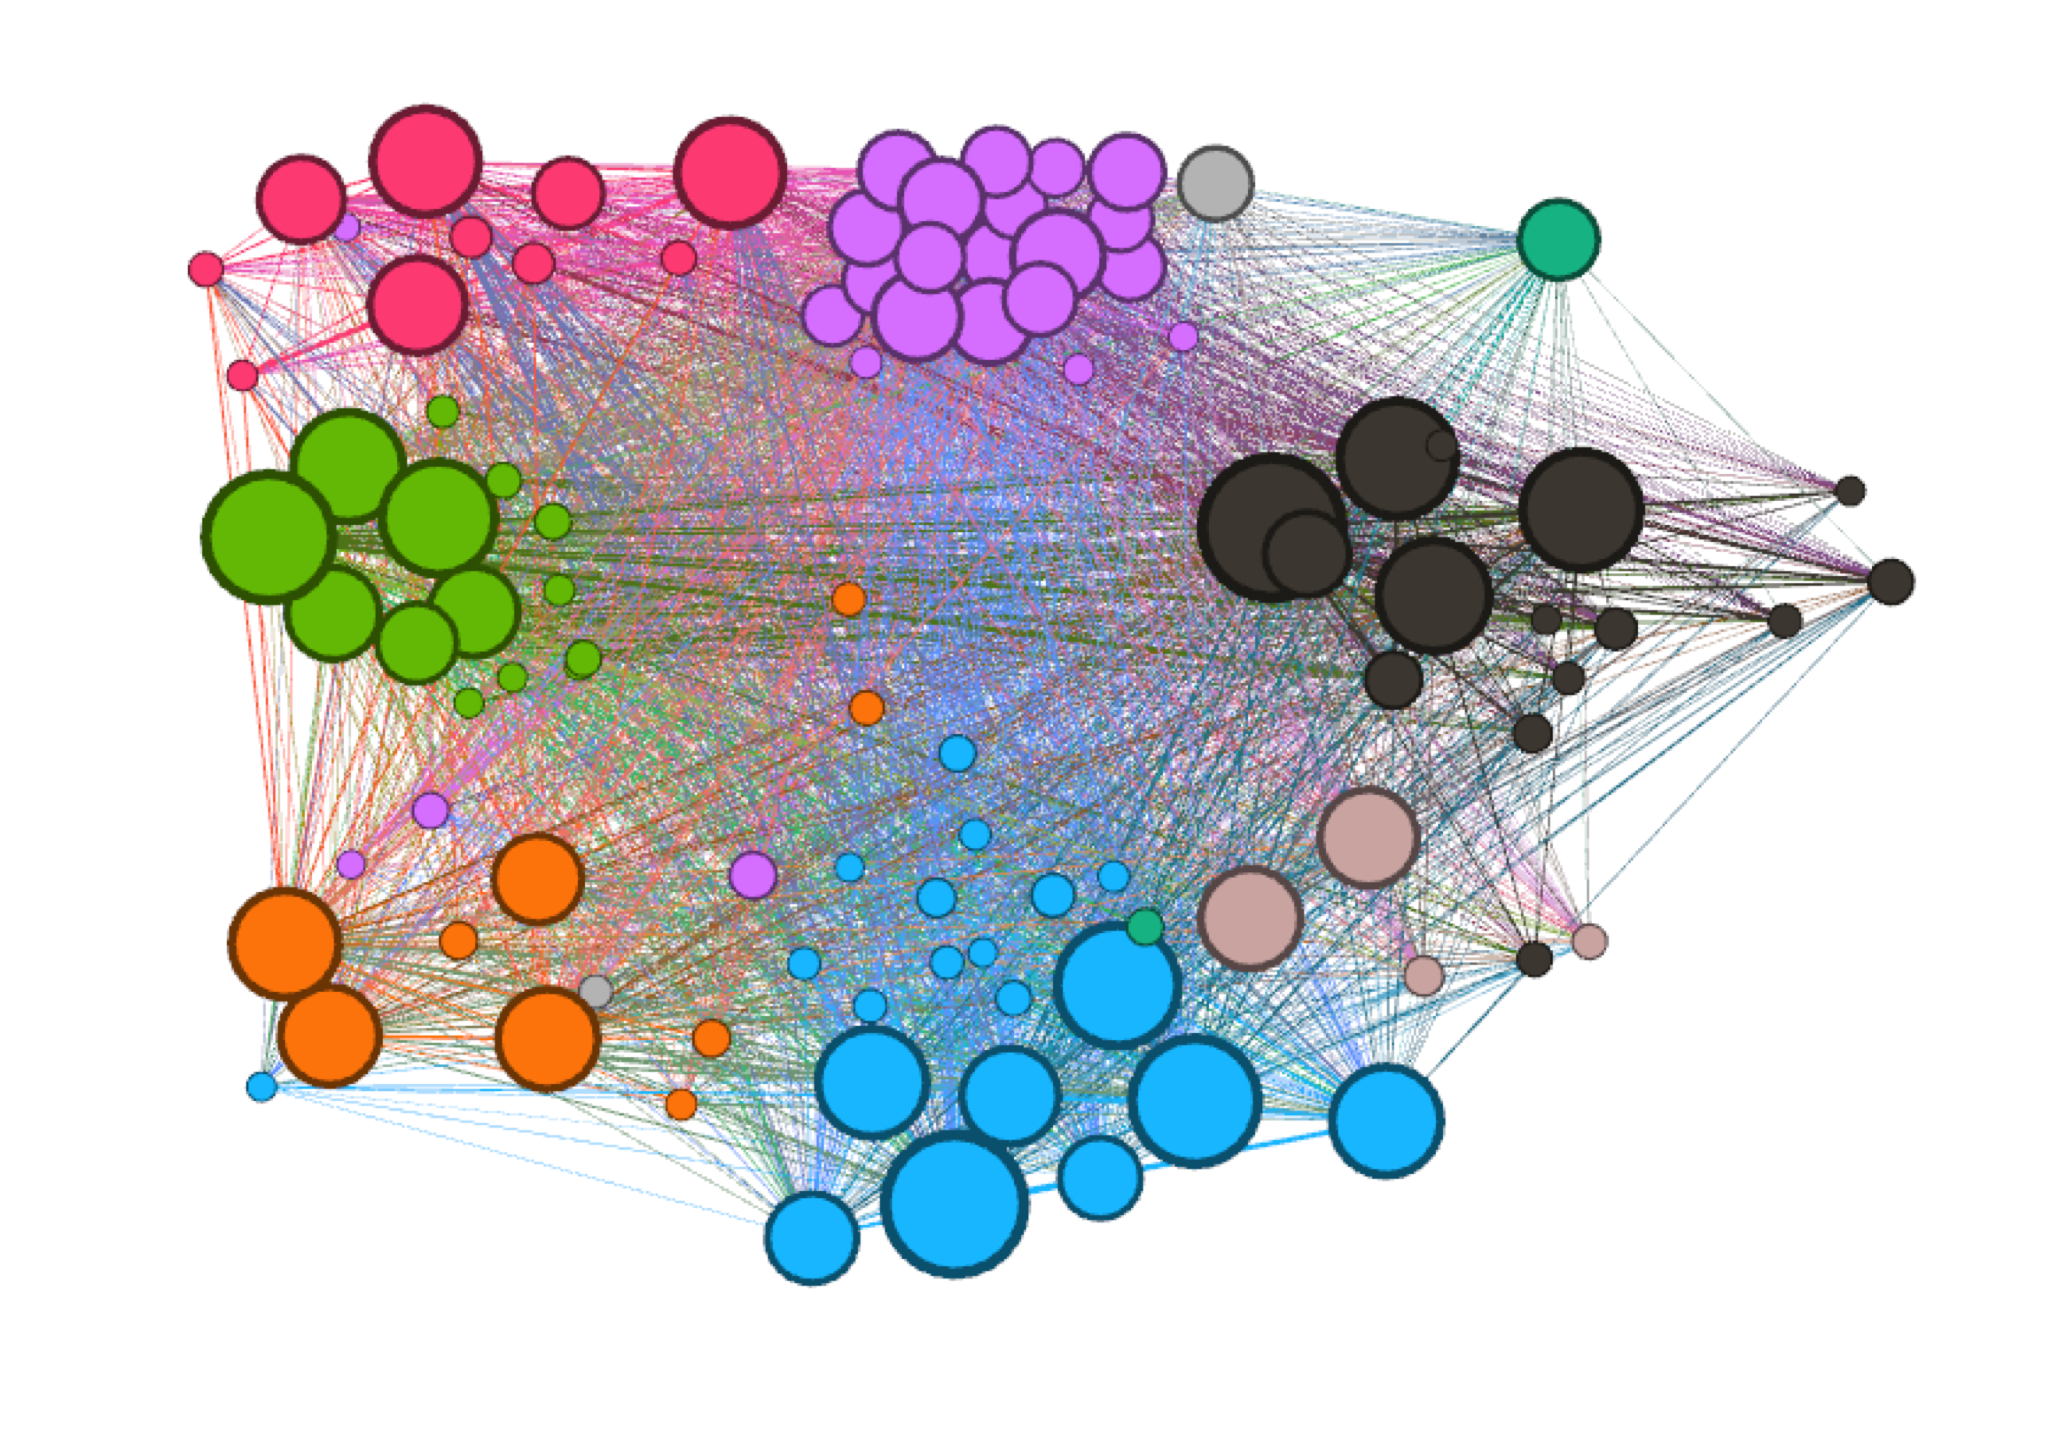
\includegraphics[width=8cm]{figure7.png}
   \caption{Example of caption.}
\end{figure}

What we did find, upon manual analysis of the data was relatively interesting. We found that despite looking at the top 150 collaborated institutions for a multitude of institutions, some remained at the top of the list across the board. Of note, the Ohio State University and Massachusetts Institute of Technology both appeared at the top, or near the top of many of the institutions in our list. We also found that institutions heavily collaborated with institutions that were highly ranked in similar fields with them. For instance, Carnegie Mellon’s papers were 34.4\% computer science papers, and their second most collaborated institution was MIT. \\

We also found that institutions tend to cite other institutions that are closer to them geographically more heavily, as one would expect. For example, CMU and University of Pittsburgh collaborated more than even CMU and MIT. Likewise, MIT and Harvard, which are both in Cambridge, Massachusetts worked together quite heavily. \\

The core metric, however, when looking at institutions continues to be that institutions number of authors. Institutions with a large number of authors tend to just have more coauthorships in general.  We somewhat accounted for this problem in the data collection method. Because our data collection was just based on the top 50 collaborating institutions for the institutions that we looked at, we were able to ensure that one institution with a very high number of publications wouldn’t be significantly biased over the others. This is because we are not looking at all their papers, but rather at the subset of papers that were worked on with their most collaborated affiliations. \\

When comparing the data across the communities, and to publically available ranking data we did garner some interesting insights. Firstly, as mentioned before, institutions with high rankings in a particular field did tend to work together more often. We looked into this further, to see if this was biased by there being a large number of papers published by those institutions in those fields, and we found that wasn’t necessarily the case. For instance, while roughly 34\% of CMU’s papers are published in the field of computer science, only about 10\% of the papers from MIT were published in that field. That hints at the notion that CMU researchers may be more inclined to work with MIT researchers, and vice versa, even though CMU publishes more computer science papers compared to its other disciplines than MIT does. \\

During milestone 3, we also looked at our institution citation data in conjunction with the ARWU university world rankings [5]. Of note, ARWU rankings claim to include publication citation data within their rankings of universities. As such, we looked at a subset of universities from their rankings, and compared it to the larger nodes within our own network. Our results were somewhat compelling. \\

When looking at ARWU rankings, we saw that high ranked institutions, namely Harvard, and MIT appeared to be collaborated with by most of our institutions. That is to say, that these very highly ranked institutions merited more collaboration across the board. We also found hits of a `rich get richer' property of these networks, so good schools tended to like to work with other good schools. In fact, a key metric is that none of the universities who appeared in our top-50 list fell out of the top 500 universities according to the ARWU.\\

In a word, these are interesting findings because it confirms what we know about the schools; they are good schools and as such professors want to work with them more often. \\

It would seem now that the prestige of the institution is a factor in authors working with one another, we are not sure of the reason for this yet. We may hypothesize that high ranked institution relationships give some credence to the findings in the paper; for example, professors are more likely to give weight to a paper with an author from Harvard.\\

From these results, we can find one simple truth; when compared against general world University Rankings, one can be sure that working with a well connected university will increase the amount of academics exposed to a paper, and will have the opportunity to work with more academics. \\

For the next milestone, we are looking at applying a page-rank like analysis to the rankings. We would like to see if position in the graph relative to high-ranking universities indicates anything about the ranking of your university. For instance, if one authors papers with primarily Harvard, does that mean that their university is also good? This will serve as a way we can predict what a university may be ranked in the future. We also want to look at other datasets in order to confirm our results like the Times international rankings. \\

Our notions of success for institutions still need some polish, but we have found that highly ranked institutions, via world rankings (from Wikipedia) tend to cite other institutions that were also highly ranked. We also found that institutions with a large number of authors found themselves at the top of the collaboration lists (like the Ohio State University.) While not explored yet, we think that filtering on paper type and institutional rankings from third party sources may give us more incite in to what makes a successful institution successful.


%-------------------------------------------------------------------------
\Section{Conclusion}
We have found now, that because we were able to gather a significant amount of data that we are beginning to see some results. Those results do somewhat differ from the results we had anticipated. For instance, the institution citation network had to include international institutions rather than just US based ones. Without internationally institutions, it would have been impossible accurately capture the collaborations that occur between institutions. International collaboration is simply much more common than we thought. \\

We did however see some results that we did expect. For instance, having a strong community structure between authors, when based on collaborations is something we did expect. That, as mentioned, derives itself from the fact that some authors worked on multiple highly popular and highly collaborated on papers. These authors became central nodes in the collaboration graphs. \\

We still feel that our metrics for success can be further refined. We must find better metrics than strong communities must, and high degrees to determine which of our nodes are truly successful, though we believe this is a good starting point.\\

Interestingly for our university data, we found what one would expect, that high ranked universities are likely to be collaborated with across the board. This could lead us in to our first unique success metric; that working with well-regarded universities as viewed by typical rankings tends to make an author more well connected. \\

Our next step in that regard should be to classify the universities more tightly, and maybe establish a ranking system that shows how many times they are cited by other high ranking universities. This may help us identify institutions are up and coming, and ones that may make a splash in college rankings. We will also produce these same results with H-index

%-------------------------------------------------------------------------
\Section{Future Work}
M3: Now that we have collected a good amount of working data, we must begin thinking more in depth how to compare success in academia. We should also look into cross correlating both H-index, and magazine rankings with our journal and institution networks. Lastly, we will work together on branching out the author subjects from just the field of astrophysics. \\

M4: Further analysis of our data from M2 left us with some interesting questions. We are now narrowing down the success metrics we might be using to view institutional and journal success. We need to apply these similar metrics to authors. We hope to be able to show by the deadline some unique metrics that will truly help us identify what success is in academia, and how to see when success will be achieved. For instance, the colocation of the universities with ‘good universities’ may be important, we also plan to do this analysis with  h-index of authors.

%-------------------------------------------------------------------------
\Section{Citations}
\relax\noindent 
 [1] Sinatra, Roberta, et al. "A century of physics." Nature Physics11.10(2015):791-796.\\
\relax
 [2] M. E. J. Newman, Phys. Rev. E 74, 036104 (2006\\
\relax
 [3] http://www.adsabs.harvard.edu/\\
\relax
 [4] http://www.scopus.com/\\
\relax
 [5] http://www.shanghairanking.com/ARWU-Statistics-2016.html\\
\relax
 [6] https://en.wikipedia.org/wiki/H-index\\
\relax
 [7] https://scholar.google.com/citations?view\_op=top\_venues\&hl=en\\

\SubSection{Footnotes}

Please use footnotes sparingly%
\footnote
   {%
     Or, better still, try to avoid footnotes altogether.  To help your
     readers, avoid using footnotes altogether and include necessary
     peripheral observations in the text (within parentheses, if you
     prefer, as in this sentence).
   }
and place them at the bottom of the column on the page on which they are
referenced. Use Times 8-point type, single-spaced.


%-------------------------------------------------------------------------
\nocite{ex1,ex2}
\bibliographystyle{latex8}
\bibliography{latex8}

\end{document}
